\documentclass[a4paper, 12pt]{report}

%%%%%%%%%%%%
% Packages %
%%%%%%%%%%%%
\usepackage{rest-api}
\usepackage[english]{babel}
\usepackage[noheader]{packages/sleek}
\usepackage{packages/sleek-title}
\usepackage{packages/sleek-theorems}
\usepackage{packages/sleek-listings}
\usepackage[most]{tcolorbox}


\usepackage{color}
\usepackage{tabularx}

\usepackage{pdfpages}

\definecolor{pblue}{rgb}{0.13,0.13,1}
\definecolor{pgreen}{rgb}{0,0.5,0}
\definecolor{pred}{rgb}{0.9,0,0}
\definecolor{pgrey}{rgb}{0.46,0.45,0.48}
\definecolor{tsyellow}{RGB}{255,185,88}

\usepackage{listings}
\lstset{language=Java,
 columns=fullflexible,
  showspaces=false,
  showtabs=false,
  frame=single,
  breaklines=true,
  postbreak=\mbox{\textcolor{red}{$\hookrightarrow$}\space},
  showstringspaces=false,
  breakatwhitespace=true,
  commentstyle=\color{pgreen},
  keywordstyle=\color{pblue},
  stringstyle=\color{pred},
  basicstyle=\ttfamily
}

\usepackage{enumitem,amssymb}

\newlist{todolist}{itemize}{2}
\setlist[todolist]{label=$\square$}

\newenvironment{boxexercise}
{\begin{tcolorbox}
[enhanced jigsaw,breakable,pad at break*=1mm,
 colback=tsyellow!20,boxrule=0pt,frame hidden]}
{\end{tcolorbox}}

\newenvironment{summary}
{\hspace{10pt}\par\small\it
 \begin{list}{}{\leftmargin=35pt\rightmargin=25pt}
 \item\ignorespaces\advance\baselineskip -1pt}
{\end{list}\vspace{-0.5cm}}

\newenvironment{remark}
{\vspace{0.5cm}\noindent\small\it
 \marginpar{\vspace{-3mm}
\includegraphics[width=1.0cm]{idea}}}
{\vspace{0.5cm}}

\newtheorem{envoefening}{\textbf{Exercise}}[chapter]
\newenvironment{oefening}
               {\begin{boxexercise}\begin{envoefening}}
               {\end{envoefening}\end{boxexercise}}
               
\newcommand*{\xml}[1]{\texttt{<#1>}}

%%%%%%%%%%%%%%
% Title-page %
%%%%%%%%%%%%%%

\logo{./resources/pdf/logo.png}
\institute{Hogeschool PXL}
\faculty{PXL-Digital}
%\department{Department of Anything but Psychology}
\title{Introduction to Spring Boot}
\author{\textit{Author}\\Nele \textsc{Custers}}
%\supervisor{Linus \textsc{Torvalds}}
%\context{Well, I was bored...}
\date{\today}

%%%%%%%%%%%%%%%%
% Bibliography %
%%%%%%%%%%%%%%%%

\usepackage{biblatex}
\addbibresource{./resources/bib/references.bib}

%%%%%%%%%%
% Others %
%%%%%%%%%%

\lstdefinestyle{latex}{
    language=TeX,
    style=default,
    %%%%%
    commentstyle=\ForestGreen,
    keywordstyle=\TrueBlue,
    stringstyle=\VeronicaPurple,
    emphstyle=\TrueBlue,
    %%%%%
    emph={LaTeX, usepackage, textit, textbf, textsc}
}

\FrameTBStyle{latex}

\def\tbs{\textbackslash}

%%%%%%%%%%%%
% Document %
%%%%%%%%%%%%

\begin{document}
    \maketitle
    \romantableofcontents


\chapter{Introduction}
    
\fcolorbox{black}[HTML]{E9F0E9}{\parbox{\textwidth}{%
\noindent \textbf{Learning goals}\\
The junior-colleague
\begin{enumerate}[nolistsep]
\item can describe what Spring is
\item can describe what Spring Boot is
\item can explain what a three-tier application is
\item can identify the three layers in a Spring Boot application
\item can explain the responsibilities of the layers in a Spring Boot application
\item can explain the architecture of a Spring RESTful web application
\item can explain what a DTO is
\item can explain what an entity-object is
\item can explain what dependency injection is
\item can explain what a Spring bean is
\item can explain what a Spring container is
\item can explain what a Spring Boot starter is
\end{enumerate}}}


\section{Enterprise Applications with Java}
By 1999, Java had developed a loyal following among application developers and Sun saw an opportunity to extend the language for traditional enterprise workloads. With the launch of J2EE, and another technology that was gaining prominence — the application server — enterprises now had a platform that was designed to meet their needs with capabilities for things like security, scalability and reliability.

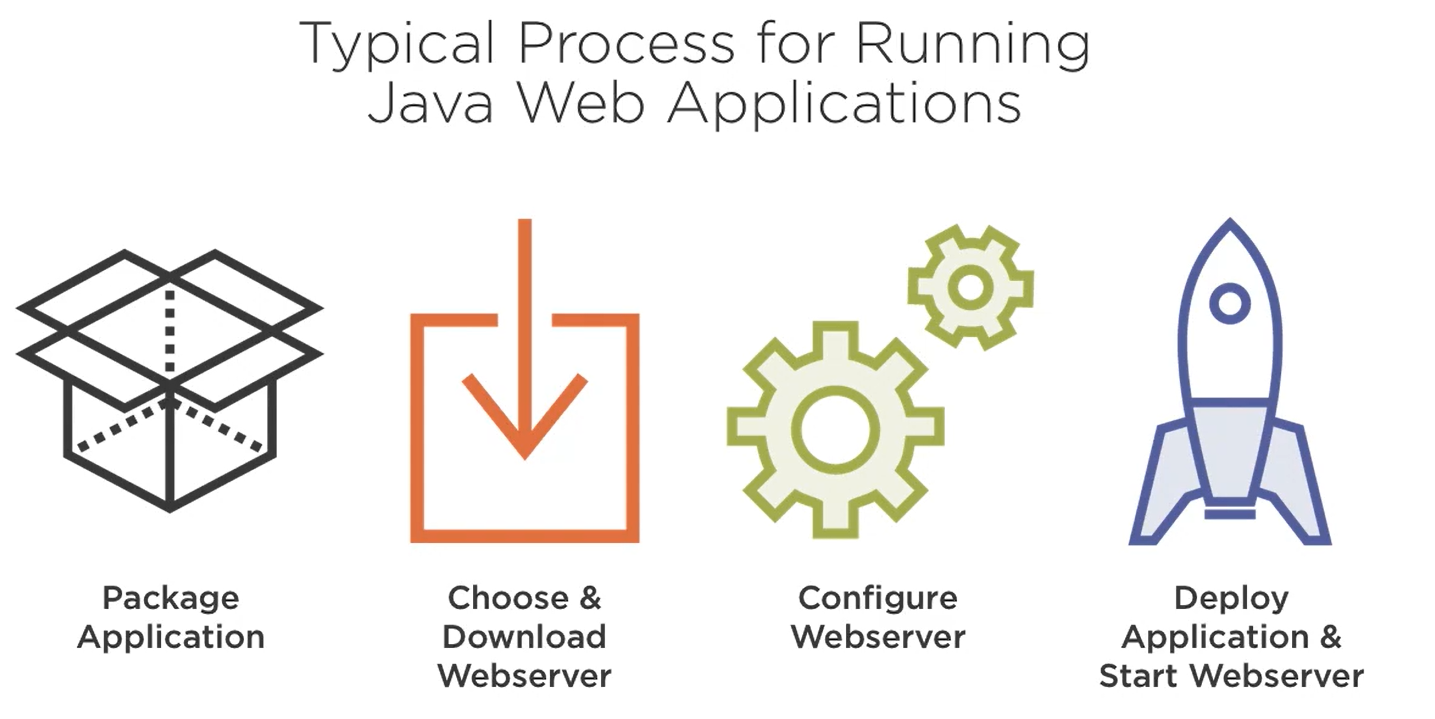
\includegraphics[width=\textwidth]{./images/chapter1/before_spring_boot.png} 

Spring came into being in 2003 as a response to the complexity of the early J2EE specifications. While some consider Java EE and its modern-day successor Jakarta EE to be in competition with Spring, they are in fact complementary. The Spring programming model does not embrace the Jakarta EE platform specification; rather, it integrates with carefully selected individual specifications from the traditional EE umbrella. Spring started as a lightweight alternative to Java Enterprise Edition. Rather than develop components as heavyweight Enterprise
JavaBeans (EJBs), Spring offered a simpler approach to enterprise Java development, utilizing dependency injection and aspect-oriented programming to achieve the capabilities of EJB with plain old Java objects (POJOs).
But while Spring was lightweight in terms of component code, it was heavyweight in terms of configuration. Initially, Spring was configured with XML (and lots of it).
It provides everything you need to create Java enterprise applications. Spring offers the flexibility to create many kinds of architectures depending on an application’s needs. As of Spring Framework 6.0, Spring requires Java 17+.

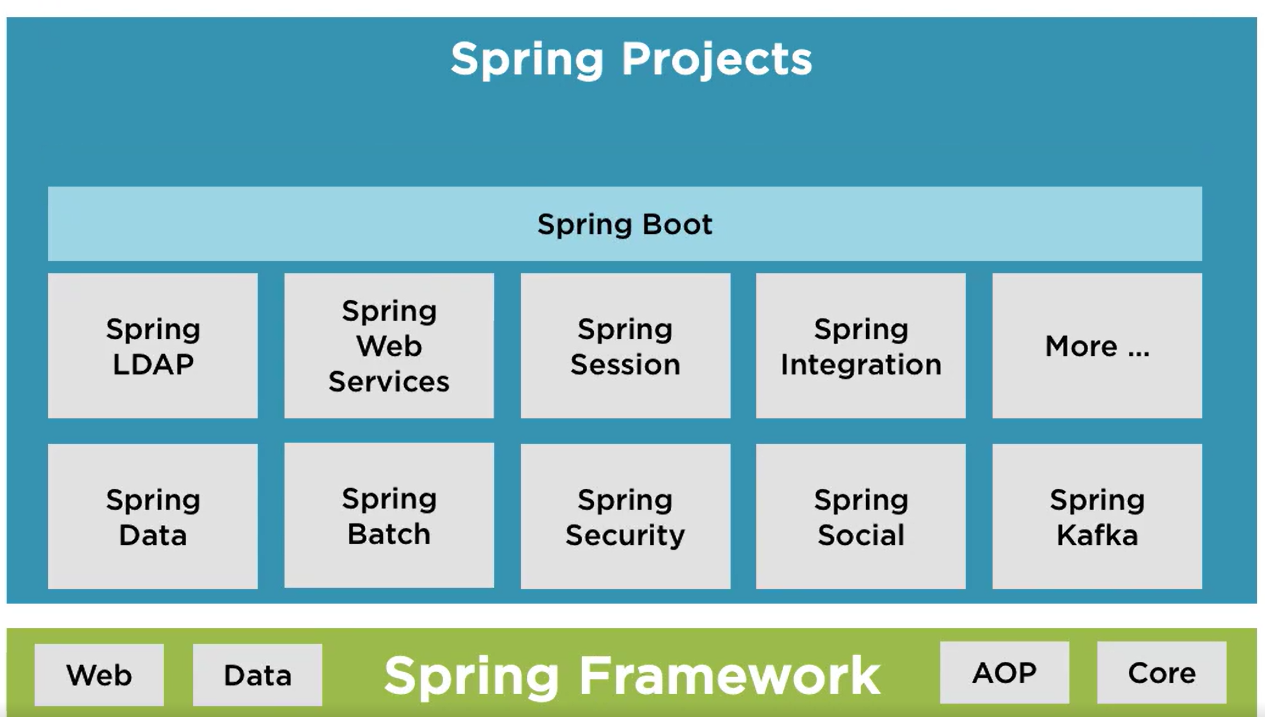
\includegraphics[width=\textwidth]{./images/chapter1/spring_framework.png} 

Spring Boot is a project that is built on the top of the Spring Framework. It provides an easier and faster way to set up, configure, and run java applications.

    
\section{What is Spring Boot?}
 
Spring Boot is an open-source Java framework to create production-ready,  standalone Spring applications. It's a robust, widely used framework. The creation of this framework was facilitated by the desire to simplify the development of applications on the popular Java EE technology stack from Oracle, which was very complex and difficult to use at the time. With very little configuration, you can create easily your first Spring Boot application.

Let's look at some advantages of Spring Boot for developers 
\begin{itemize}
\item speed up the process of creating and deploying application
\item create standalone applications with less or almost no configuration overhead
\item easy to learn framework
\item increase productivity of developers
\end{itemize}

\section{Bootstrapping a simple application}

\subsection{Using Spring Initializr}
Spring Initializr is a web application that can generate a Spring Boot project.
The url for this web application is \url{https://start.spring.io/}. You can select the necessary configuration, including the build tool, language, version of the Spring Boot framework, and any dependencies for your project. IntelliJ IDEA Ultimate provides the Spring Initializr project wizard that integrates with the Spring Initializr API to generate and import your project directly from the IDE.

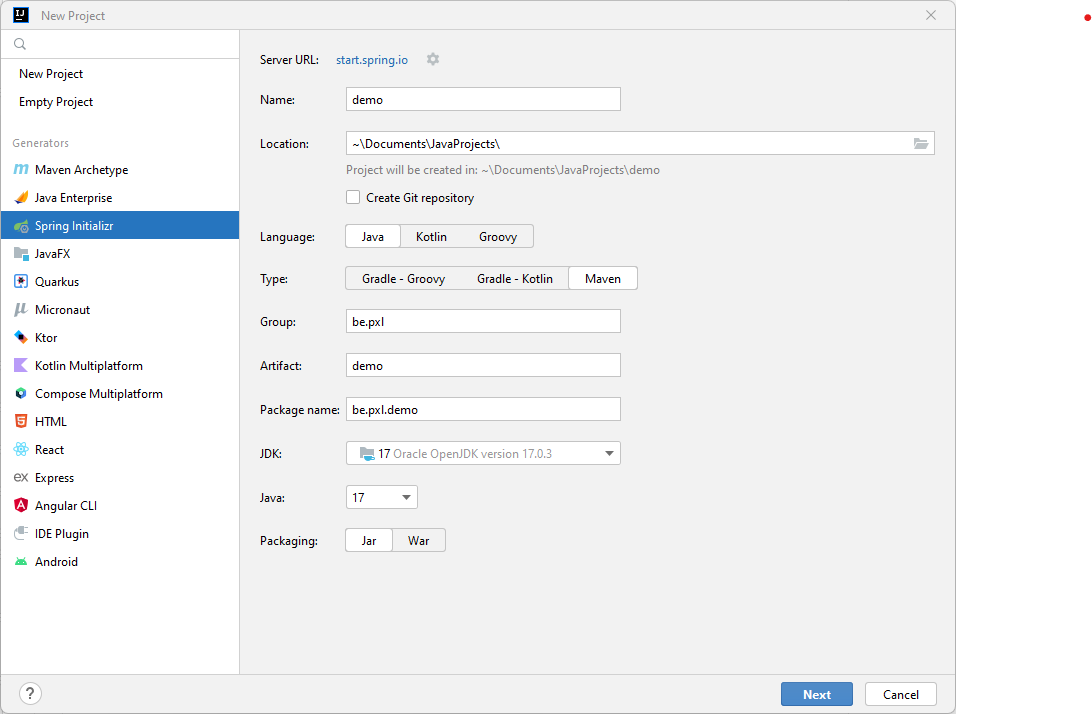
\includegraphics[width=\textwidth]{./images/chapter1/spring_initializer_intellij.png}

\includegraphics[width=\textwidth]{./images/chapter1/new_project.png}

We select Spring Web dependency. Spring Web uses Spring MVC. It is used for building RESTful Web Services. Spring MVC provides the annotation @RestController for classes that implement the REST endpoints.
To run a RESTful Web Service you need a web container. Spring Boot will automatically add an embedded Tomcat web container to your project. If you prefer another web container, you can update Spring Boot's configuration.
Finally Jackson is a popular third-party library for converting Java-objects to JSON and vice versa.

\begin{oefening}
Create the demo project. You can use the wizard in IntelliJ IDEA Ultimate or \url{https://start.spring.io/}.
\end{oefening}

\section{Running the demo project}

The starting point of a Spring Boot application is the class with the main-method and annotated with @SpringBootApplication.  This class can be found in the folder /src/main/java.  Spring Boot offers a lot of annotations to reduce the workload of developers.   

\begin{lstlisting}[frame=single]
package be.pxl.demo;

import org.springframework.boot.SpringApplication;
import org.springframework.boot.autoconfigure.SpringBootApplication;

@SpringBootApplication
public class DemoApplication {

    public static void main(String[] args) {
        SpringApplication.run(DemoApplication.class, args);
    }

}
\end{lstlisting}

By running the main-class you start your Spring Boot application. 

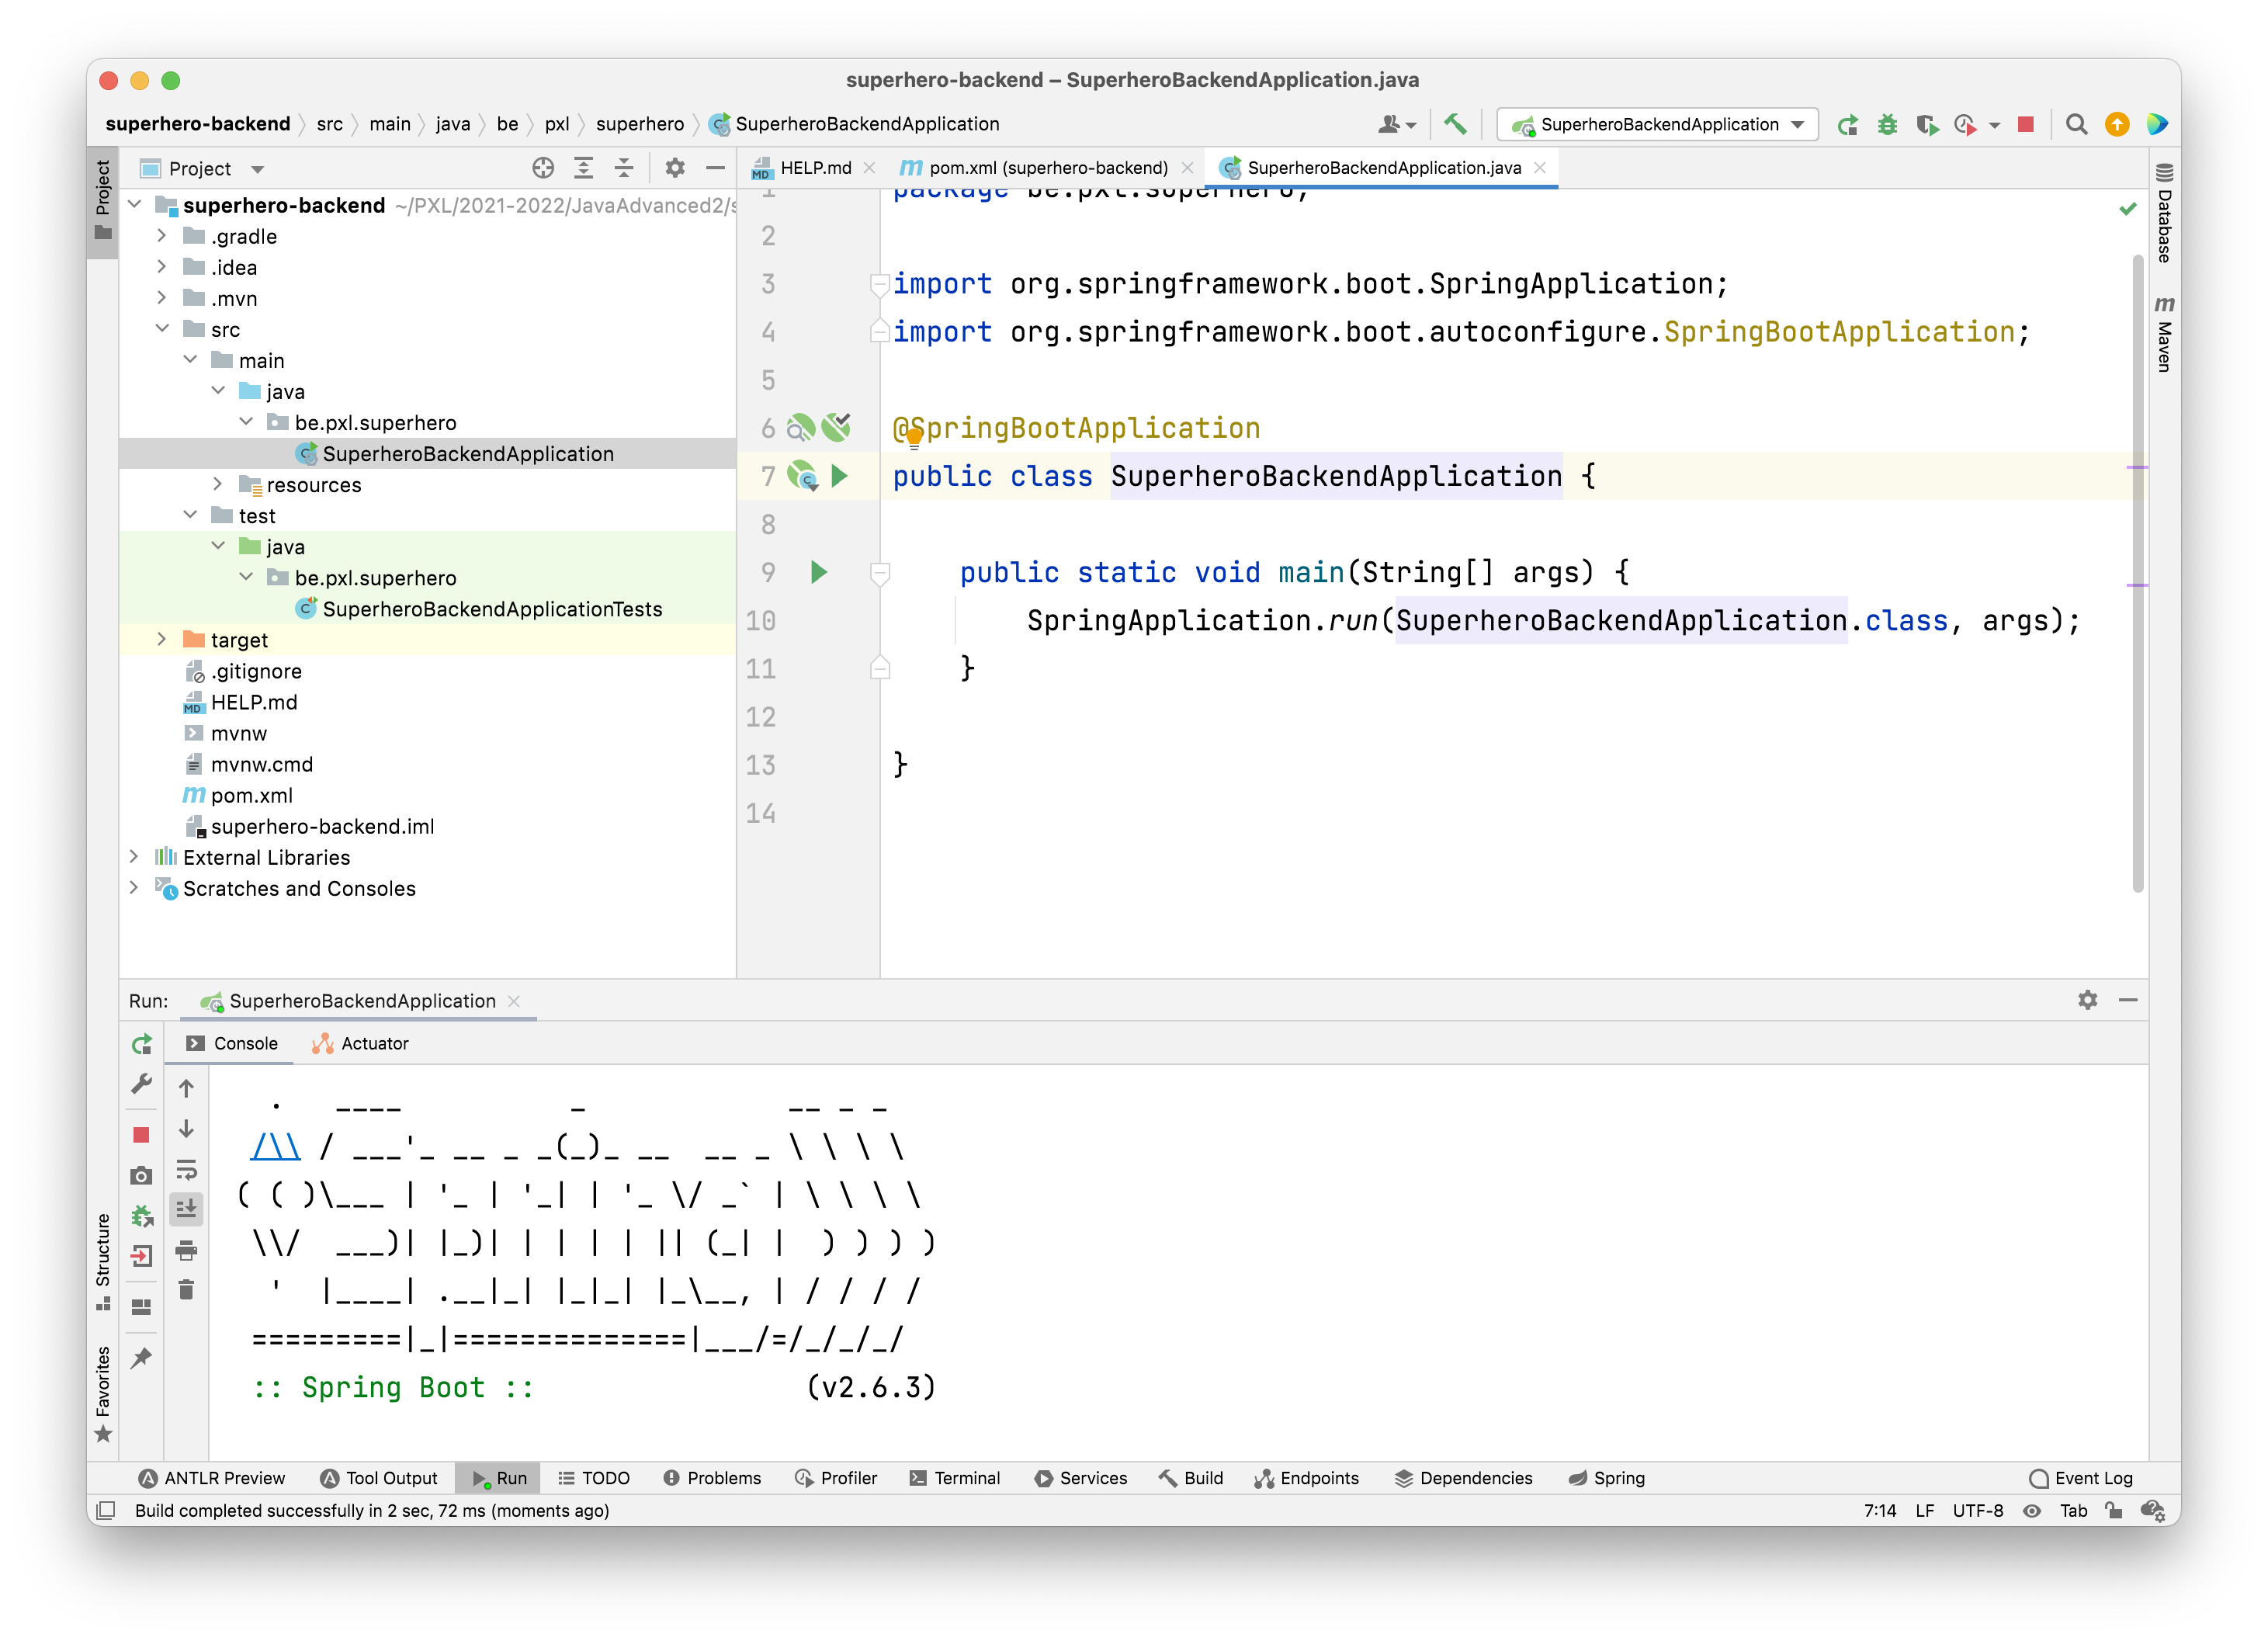
\includegraphics[width=\textwidth]{./images/chapter2/first-run.png}

Currently our Spring Boot application only shows a whitelabel error page. This error page is available when you perform a GET for URL \url{http://localhost:8080}.

\frame{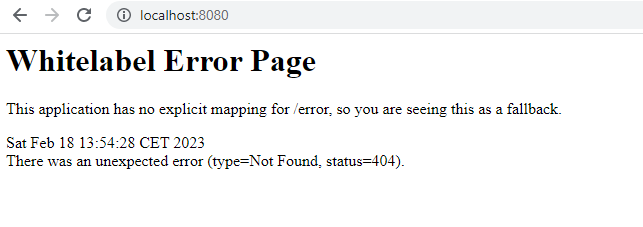
\includegraphics[width=\textwidth]{./images/chapter2/whitelabel_error_page.png}} 

Port 8080 is the default port. If this port is not available you will see an error message in Spring Boot's logging.

\begin{lstlisting}[frame=single]
***************************
APPLICATION FAILED TO START
***************************

Description:

Web server failed to start. Port 8080 was already in use.
\end{lstlisting}

The port number can be changed in the file application.properties. You have to add the property server.port here with the desired port number.

\begin{lstlisting}[frame=single]
server.port=8081
\end{lstlisting}

\subsection{The Maven pom file}

POM stands for \'Project Object Model\'. It is an XML representation of a Maven project held in a file named pom.xml. This file can be found in your project directory. The POM contains all necessary information about a project, as well as configurations of plugins to be used during the build process. We will cover Maven in chapter 3.

\begin{lstlisting}[frame=single]
<?xml version="1.0" encoding="UTF-8"?>
<project xmlns="http://maven.apache.org/POM/4.0.0" xmlns:xsi="http://www.w3.org/2001/XMLSchema-instance"
         xsi:schemaLocation="http://maven.apache.org/POM/4.0.0 https://maven.apache.org/xsd/maven-4.0.0.xsd">
    <modelVersion>4.0.0</modelVersion>
    <parent>
        <groupId>org.springframework.boot</groupId>
        <artifactId>spring-boot-starter-parent</artifactId>
        <version>3.0.2</version>
        <relativePath/> <!-- lookup parent from repository -->
    </parent>
    <groupId>be.pxl</groupId>
    <artifactId>demo</artifactId>
    <version>0.0.1-SNAPSHOT</version>
    <name>demo</name>
    <description>demo</description>
    <properties>
        <java.version>17</java.version>
    </properties>
    <dependencies>
        <dependency>
            <groupId>org.springframework.boot</groupId>
            <artifactId>spring-boot-starter-web</artifactId>
        </dependency>

        <dependency>
            <groupId>org.springframework.boot</groupId>
            <artifactId>spring-boot-starter-test</artifactId>
            <scope>test</scope>
        </dependency>
    </dependencies>

    <build>
        <plugins>
            <plugin>
                <groupId>org.springframework.boot</groupId>
                <artifactId>spring-boot-maven-plugin</artifactId>
            </plugin>
        </plugins>
    </build>
</project>
\end{lstlisting}

spring-boot-starter-parent is a starter project that provides the default configuration for spring-based applications. Here you choose the version of Spring Boot.

For large projects, managing the dependencies is not always easy. Spring Boot solves this problem by grouping certain dependencies together. These groups of dependencies are called starters. All Spring Boot starters are named following the same naming pattern. The all start with spring-boot-starter-*, where * indicates the purpose and functionality provided by the starter.

spring-boot-starter-web adds all the libraries we need to develop web components. An embedded server will be provided in the Spring Boot project. Therefore the environment where the Spring Boot project is executed does not need to have a pre-installed server. The default embedded server for Spring Boot is Tomcat. The Spring MVC framework which provides all classes for developing RESTful web services is also part of spring-boot-starter-web.

spring-boot-starter-test (with scope test) is the starter for testing Spring Boot applications with libraries including JUnit Jupiter, Hamcrest and Mockito.

\subsection{A Rest Controller}

RestControllers are used for making RESTful web services with the help of the @RestController annotation. The RestController allows to handle all HTTP methods such as GET, POST, DELETE, PUT. 

\begin{lstlisting}[frame=single]
package be.pxl.demo.api;

import jakarta.annotation.PostConstruct;
import org.springframework.web.bind.annotation.GetMapping;
import org.springframework.web.bind.annotation.RestController;

import java.util.ArrayList;
import java.util.List;
import java.util.Random;

@RestController
public class GreetingController {

    private final List<String> messages = new ArrayList<>();
    private static final Random RANDOM = new Random();

    @PostConstruct
    public void init() {
        messages.add("Peek-a-boo!");
        messages.add("Howdy-doody!");
        messages.add("My name's Ralph, and I'm a bad guy.");
        messages.add("I come in peace!");
        messages.add("Put that cookie down!");

    }

    @GetMapping("/hello")
    public String doGreeting() {
        return messages.get(RANDOM.nextInt(messages.size()));
    }
}
\end{lstlisting}

When Spring's DispatcherServlet receives a request for the URL /hello it looks for the correct @RestController to handle the request. The annotation @RequestMapping is used for mapping all incoming HTTP request URLs to the corresponding controller methods. The DispatcherServlet will be discussed in detail in a later chapter. The Spring container is responsible for managing an instance of the @RestController. When an instance of our GreetingController is created,  the init method is called to initialise all possible greetings.  The @GetMapping is a specialized version of @RequestMapping and is used for methods handling HTTP  GET requests.  Therefore, when we call the URL \url{http://localhost:8080/hello}, the method doGreeting() in the GreetingController will handle the request and return a greeting message in text format.

\begin{oefening}
Create the package \textit{be.pxl.demo.api}. Add the class \textbf{GreetingController} in this package. Restart the Spring Boot application and open the URL \url{http://localhost:8080/hello} in a browser.
\end{oefening}

\subsection{Auto-configuration}

Spring Boot auto-configuration attempts to automatically configure your Spring application based on the dependencies that you have added.
To gain some insight in this auto-configuration let's add a line in the application.properties file. This file can be found in the directory /src/main/resources. 

\begin{lstlisting}
logging.level.org.springframework=debug
\end{lstlisting}

logging.level.org.springframework is a application properties. A list of all available application properties can be found at \url{https://docs.spring.io/spring-boot/docs/current/reference/html/application-properties.html}.

\begin{oefening}
Add the line above to the application.properties file and restart the Spring Boot application.
\end{oefening}

In the console you will find all the auto-configuration Spring Boot is doing.

\subsection{@SpringBootApplication}

Java annotations are a mechanism for adding metadata information to our source code. An annotation processor processes these annotations at compile time or runtime to provide functionality such as code generation, error checking, etc.

@SpringBootApplication annotation is used to enable following three features:
\begin{itemize}
\item @EnableAutoConfiguration: enable Spring Boot’s auto-configuration mechanism
\item @ComponentScan: enable @Component scan on the package where the application is located
\item @Configuration: allow to register extra beans in the context or import additional configuration classes
\end{itemize}


\section{Components and dependency injection}

All our REST backend applications will consist of 3 layers:
 router-layer (or API-layer), service- or business-layer and persistence-layer.

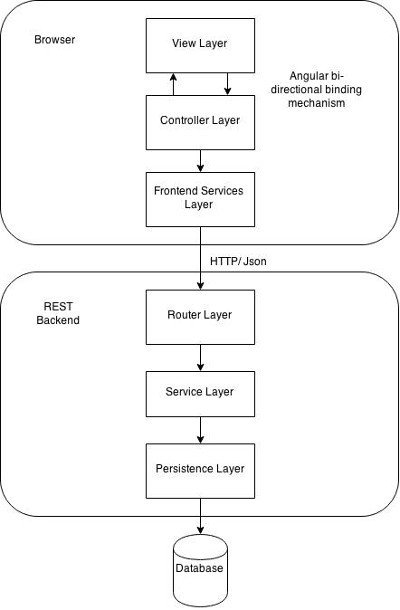
\includegraphics[scale=0.6]{./images/chapter1/spring-architecture.jpeg} 

\begin{itemize}
\item \textbf{Router- or presentation layer:}  Handling and processing HTTP requests,  translating JSON parameters to objects,  authentication of users and protecting data from maleficent users,  ... .
\item \textbf{Service- or business logic layer:} This layer contains the business logic, the core functionality of your application. All calculations, decisions, evaluations, data processing,... are handled by this layer. 
\item \textbf{Data- or persistence layer:} This layer is responsible for interacting with the database.  This layer stores and retrieves the application data in the database.
\end{itemize}

The typical components for each layer are annotated.  These annotated components are managed by Spring. Developers are not responsible for creating the objects of these component classes. The actual objects are created and injected by Spring wherever we need them. In later chapters we will discuss the concept of dependency injection in detail.

The annotations for the Spring components we will use are:
\begin{itemize}
\item @Component: generic annotation for all components managed by Spring
\item @RestController: indicate the components in the API layer
\item @Service: indicate the components in the service layer
\item @Repository: indicate the components in the persistence layer
\end{itemize}

All of these application components (@Component, @Service, @Repository, @Controller, and others) are automatically registered as Spring Beans.

Here is the definition of beans from the Spring framework documentation:

\fcolorbox{black}[HTML]{E9F0E9}{\parbox{\textwidth}{%
\noindent In Spring, the objects that form the backbone of your application and that are managed by the Spring IoC container are called beans. A bean is an object that is instantiated, assembled, and otherwise managed by a Spring IoC container.}}

IoC or Inversion of Control is the process in which an object defines its dependencies without creating them. The IoC container is responsible for constructing the dependencies.

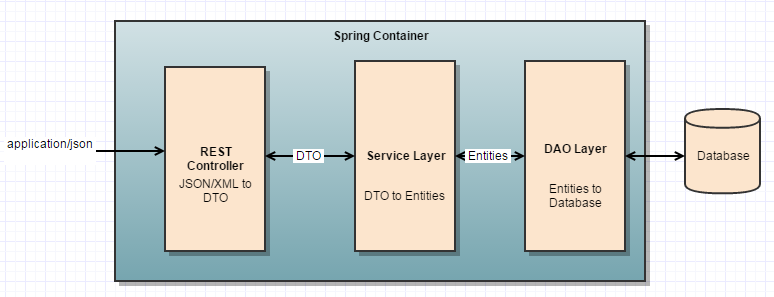
\includegraphics[width=\textwidth]{./images/Spring-REST-Web-Services.png} 

The image shows all the layers that we develop in our REST backend applications. The RestController in the API layer provides REST endpoints. The API layer communicates via DTOs or Data Transfer Objects with the service layer. The service layer implements all business logic. DTOs are mapped to entity-objects and passed along the persistence layer. The persistence layer is responsible for storing the entity-objects in the database.

The Spring container is at the core of the Spring Framework. The container is responsible for creating and managing the objects for classes annotated with @Service, @Repository,... The container will provide these objects (beans) when they are needed by other beans.


\section{DevOps Tools for Java Developers}

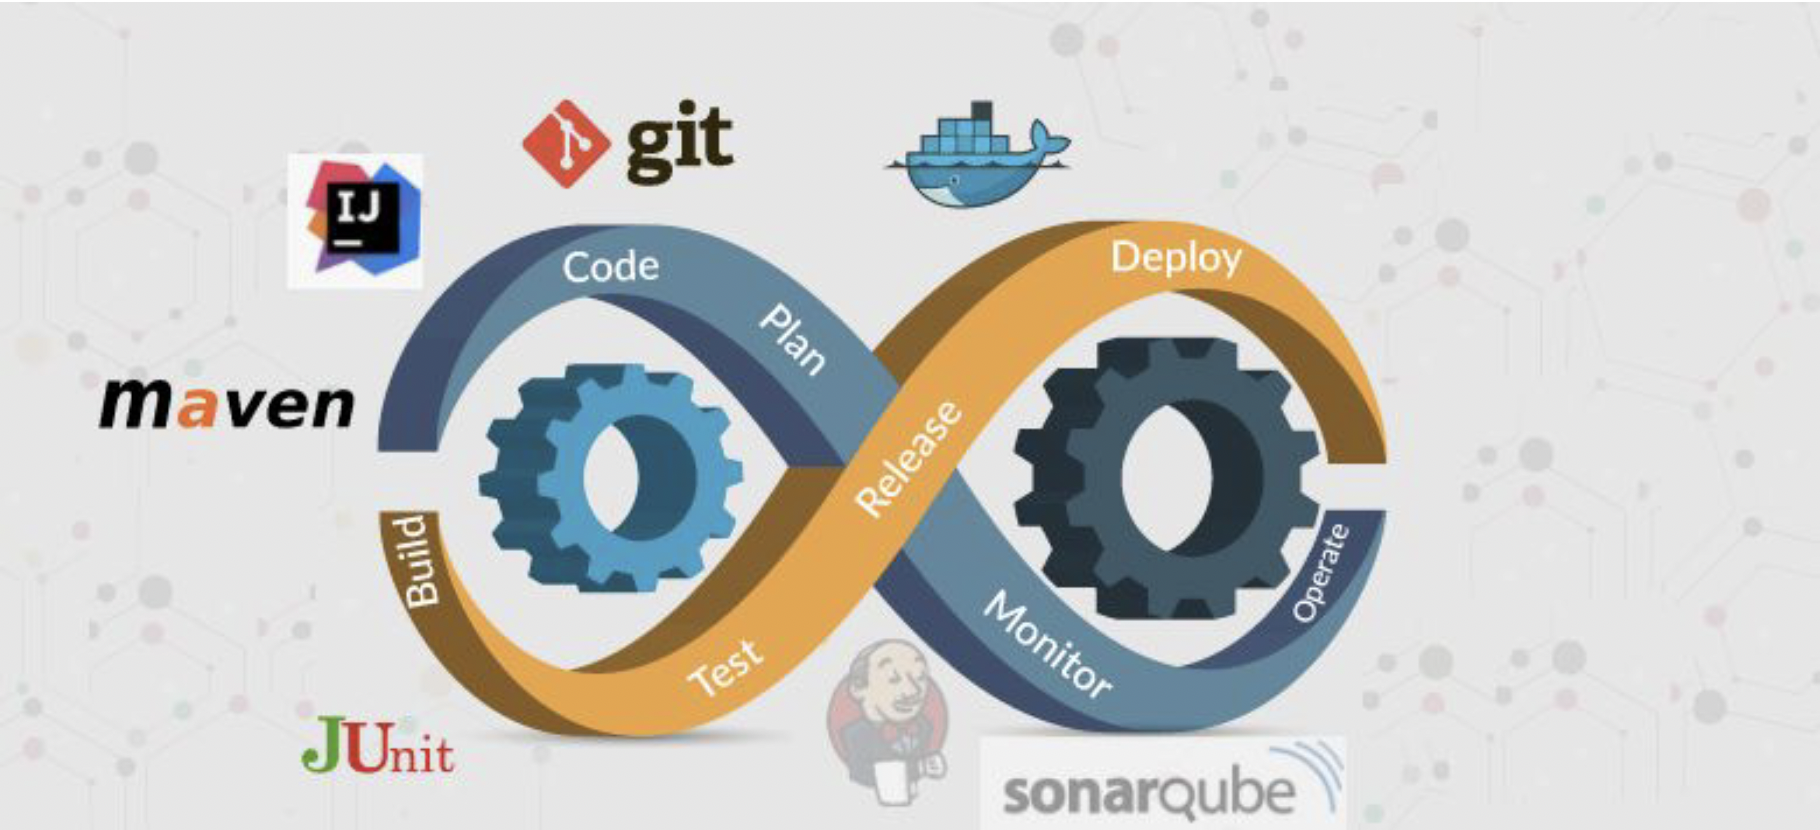
\includegraphics[width=\textwidth]{./images/chapter1/devops.png}  
 

\chapter{Creating a Spring Boot application}

\fcolorbox{black}[HTML]{E9F0E9}{\parbox{\textwidth}{%
\noindent \textbf{Learning goals}\\
The junior-colleague
\begin{enumerate}[nolistsep]
\item can identify the different components in a Spring Boot application
\item can explain what REST is
\item can explain what an entity-class is
\item can create a RestController
\item can run a Spring Boot application
\item can enable CORS support in a Spring Boot application
\item ...
\end{enumerate}}}


\section{Creating a Spring Boot project}

This chapter will guide you through the implementation of your first Spring Boot application. You will create a RESTful webservice for managing the information of a ``Super Hero Company''. We will implement REST endpoints for creating, updating and deleting superheroes. Later you will add functionality to create, update and delete missions for the superheroes.

We use Spring Intializr to bootstrap this Spring Boot application. 

\includegraphics[width=\textwidth]{./images/chapter2/new_project.png} 

In the first screen of the wizard you have to provide metadata about your project.  The information you have to provide is:
\begin{itemize}
\item \textbf{Group:} unique identification of your project across all projects.  A group follows Java's package name rules. It also infers the root package name to use.
\item \textbf{Artifact:} the name of a project artifact without version.  It also infers the name of the project.
\item \textbf{Name:} display name of the project that also determines the name of your Spring Boot application. For instance,  if the name of your project is my-app, the generated project will have a MyAppApplication class
\item \textbf{Description:} description of the project.
\item \textbf{Package Name:} root package of the project. If not specified, the value of the group attribute is used
\item \textbf{Packaging:} project packaging.  You can choose either jar or war projects.
\item \textbf{Java Version:} the Java version to use
\item \textbf{Language:} the programming language to use
\end{itemize}

During this course we use Maven as build tool for our projects. In the next chapter we will discuss Maven into detail.

Our backend provides a REST API. A clear explanation about REST can be found at \href{https://www.codecademy.com/article/what-is-rest.}{codecademy}.  To implement REST endpoints we need some third-party libraries: Spring MVC, Tomcat and Jackson. All these libraries are bundled in one starter: \textbf{spring-boot-starter-web}.

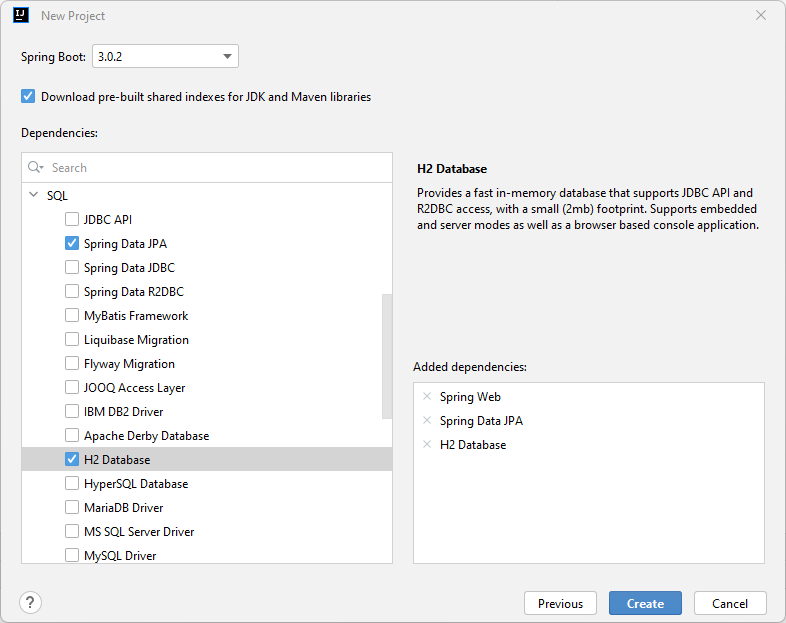
\includegraphics[width=\textwidth]{./images/chapter2/new_project_metadata.png}

Besides Spring Web, we add Spring Data JPA to the project. Using this starter depencency we can use JPA (the Java or Jakarta Persistence API) to access a database. 
The dependency spring-boot-starter-data-jpa will be added to the pom.xml file. This one starter adds different libraries for easily accessing a database.
Finaly the H2 Database dependency is added. This is an in-memory database 
and you need zero configuration to use this database. This is nice for fast prototyping, but all your data is lost once you restart the application. All database related technologies will be explained in detail during this course. 

\begin{oefening}
Create your superhero Spring Boot project. You can use the wizard in IntelliJ IDEA Ultimate or \url{https://start.spring.io/}.
\end{oefening}

\section{Storing and retrieving data}

\subsection{Entity-class Superhero}

First we need a class for respresenting the objects that are stored and retrieved from the database. Each object of this class will represent one row of a table in the relational database.
We implement the class Superhero. To save Superhero-objects to the database and retrieve Superhero-objects from the database, we annotate this class and make it an entity-class. 


\includegraphics[scale=0.5]{./images/chapter2/superman.jpeg} 

Here is the entity-class Superhero:

\begin{lstlisting}[frame=single]
package be.pxl.superhero.domain;

import jakarta.persistence.Entity;
import jakarta.persistence.GeneratedValue;
import jakarta.persistence.GenerationType;
import jakarta.persistence.Id;
import jakarta.persistence.Table;

@Entity
@Table(name="superheroes")
public class Superhero {
	
	@Id
	@GeneratedValue(strategy = GenerationType.IDENTITY)
	private Long id;
	
	private String firstName;
	private String lastName;
	private String superheroName;

	public Superhero() {
		// JPA only
	}

	public Superhero(String firstName, String lastName, String superheroName) {
		this.firstName = firstName;
		this.lastName = lastName;
		this.superheroName = superheroName;
	}

	public Long getId() {
		return id;
	}

	public String getFirstName() {
		return firstName;
	}

	public void setFirstName(String firstName) {
		this.firstName = firstName;
	}

	public String getLastName() {
		return lastName;
	}

	public void setLastName(String lastName) {
		this.lastName = lastName;
	}

	public String getSuperheroName() {
		return superheroName;
	}

	public void setSuperheroName(String superheroName) {
		this.superheroName = superheroName;
	}

	@Override
	public String toString() {
		return superheroName;
	}
}
\end{lstlisting}

The annotation @Entity indicates that the class is actually an entity-class.  Spring is able to automatically generate the database table (superheroes) with all its fields in the H2 database. 
The primary key of the table is marked with the annotation @Id.  Further, with the annotation @GeneratedValue(strategy = GenerationType.IDENTITY) we don't have to assign the primary keys to the objects. The database itself is responsible for generating and assigning the primary keys.

\begin{oefening}
Add the entity class Superhero to your project.  Create the package package \textit{be.pxl.superhero.domain} for this class.
\end{oefening}

\subsection{Repository}

To execute queries in the database we need an extra class (or interface) called a \textbf{repository}. Spring is able to automatically generate database queries. When you extend the interface JpaRepository, simple queries are already available without writing one line of code. 
The generic interface JpaRepository only needs to know which data it must store and retrieve.
Therefore it needs to know the name of the entity-class and the data type of the primary key of the entity-class. 

\begin{lstlisting}[frame=single]
package be.pxl.superhero.repository;

import be.pxl.superhero.domain.Superhero;
import org.springframework.data.jpa.repository.JpaRepository;
import org.springframework.stereotype.Repository;

@Repository
public interface SuperheroRepository extends JpaRepository<Superhero, Long> {
}
\end{lstlisting}

When you open the documentation of the generic interface JpaRepository, you can see which functionality is available for the developer.

\begin{oefening}
Add the repository-interface SuperheroRepository to the project.  Create the package  \textit{be.pxl.superhero.repository} for this interface.
\end{oefening}

\subsection{Service-layer}

The classes in the service-layer are responsible for the business logic. These classes use the repositories to save and retrieve data from the database.  It is good practice to provide an interface for every class in the service-layer (service-class). 
The service-classes may never return entity-objects. We need DTOs (Data Transfer Objects) to pass data from the service-layer to the API-layer.

\begin{lstlisting}[frame=single]
package be.pxl.superhero.service;

import be.pxl.superhero.api.SuperheroDTO;
import be.pxl.superhero.api.SuperheroRequest;

import java.util.List;

public interface SuperheroService {

	List<SuperheroDTO> findAllSuperheroes();

	SuperheroDTO findSuperheroById(Long superheroId);

	Long createSuperhero(SuperheroRequest superheroRequest);

	SuperheroDTO updateSuperhero(Long superheroId, SuperheroRequest superheroRequest);

	boolean deleteSuperhero(Long superheroId);
}
\end{lstlisting}


\begin{lstlisting}[frame=single]
package be.pxl.superhero.api;

import be.pxl.superhero.domain.Superhero;

public class SuperheroDTO {

	private final Long id;
	private final String firstName;
    private final String lastName;
    private final String superheroName;

    public SuperheroDTO(Superhero superhero) {
	   this.id = superhero.getId();
        this.firstName = superhero.getFirstName();
        this.lastName = superhero.getLastName();
        this.superheroName = superhero.getSuperheroName();
    }

	public Long getId() {
		return id;
	}

	public String getFirstName() {
        return firstName;
    }

    public String getLastName() {
        return lastName;
    }

    public String getSuperheroName() {
        return superheroName;
    }

}
\end{lstlisting}

\begin{lstlisting}[frame=single]
package be.pxl.superhero.api;

public class SuperheroRequest {

	private String firstName;
	private String lastName;
	private String superheroName;

	public SuperheroRequest(String firstName, String lastName, String superheroName) {
		this.firstName = firstName;
		this.lastName = lastName;
		this.superheroName = superheroName;
	}

	public String getFirstName() {
		return firstName;
	}

	public void setFirstName(String firstName) {
		this.firstName = firstName;
	}

	public String getLastName() {
		return lastName;
	}

	public void setLastName(String lastName) {
		this.lastName = lastName;
	}

	public String getSuperheroName() {
		return superheroName;
	}

	public void setSuperheroName(String superheroName) {
		this.superheroName = superheroName;
	}

}

\end{lstlisting}

The class SuperheroServiceImpl, annotated with @Service, provides the implementation for the interface SuperheroService.
All CRUD-operations (create-read-update-delete) for Superhero-objects are provided here.
In the class SuperheroServiceImpl all business logic can be implemented.  If we, for example, have to check that the superheroname of a superhero is unique, this class is the place to implement these checks.  (At the moment we will not yet implement this business rule!)

The SuperheroRepository is autowired in the SuperheroServiceImpl. Hence the service-class can save and retrieve data from the database with the help from this repository. 


\begin{lstlisting}[frame=single]
package be.pxl.superhero.service.impl;

import be.pxl.superhero.api.SuperheroDTO;
import be.pxl.superhero.api.SuperheroRequest;
import be.pxl.superhero.domain.Superhero;
import be.pxl.superhero.exception.ResourceNotFoundException;
import be.pxl.superhero.repository.SuperheroRepository;
import be.pxl.superhero.service.SuperheroService;
import org.springframework.stereotype.Service;

import java.util.List;
import java.util.stream.Collectors;

@Service
public class SuperheroServiceImpl implements SuperheroService {

	private final SuperheroRepository superheroRepository;

	public SuperheroServiceImpl(SuperheroRepository superheroRepository) {
		this.superheroRepository = superheroRepository;
	}

	public List<SuperheroDTO> findAllSuperheroes() {
		return superheroRepository.findAll()
				.stream().map(SuperheroDTO::new)
				.toList();
	}

	public SuperheroDTO findSuperheroById(Long superheroId) {
		return superheroRepository.findById(superheroId)
		         .map(SuperheroDTO::new)
				.orElseThrow(() -> new ResourceNotFoundException("Superhero", "ID", superheroId));
	}

	public Long createSuperhero(SuperheroRequest superheroRequest) {
		Superhero superhero = new Superhero();
		superhero.setFirstName(superheroRequest.getFirstName());
		superhero.setLastName(superheroRequest.getLastName());
		superhero.setSuperheroName(superheroRequest.getSuperheroName());
		Superhero newSuperhero = superheroRepository.save(superhero);
		return newSuperhero.getId();
	}

	public SuperheroDTO updateSuperhero(Long superheroId, SuperheroRequest superheroRequest) {
		return superheroRepository.findById(superheroId).map(superhero -> {
			superhero.setFirstName(superheroRequest.getFirstName());
			superhero.setLastName(superheroRequest.getLastName());
			superhero.setSuperheroName(superheroRequest.getSuperheroName());
			return new SuperheroDTO(superheroRepository.save(superhero));
		}).orElseThrow(() -> new ResourceNotFoundException("Superhero", "id", superheroId));
	}

	public boolean deleteSuperhero(Long superheroId) {
		return superheroRepository.findById(superheroId)
				.map(superhero -> {
					superheroRepository.delete(superhero);
					return true;
				}).orElseThrow(() -> new ResourceNotFoundException("Superhero", "id", superheroId));

	}
}
\end{lstlisting}

\begin{lstlisting}
package be.pxl.superhero.exception;

public class ResourceNotFoundException extends RuntimeException {
    public ResourceNotFoundException(String resource, String field, String value) {
        super("Not found: " + resource + " with " + field + "=" + value);
    }

    public ResourceNotFoundException(String resource, String field, long value) {
        this(resource, field, Long.toString(value));
    }
}
\end{lstlisting}

\begin{oefening}
Create the package \textit{be.pxl.superhero.api} and add the request-object SuperheroRequest and the DTO SuperheroDTO.  These classes are used for communication with the API-layer. 
Add the interface SuperheroService en the implementation SuperheroServiceImpl to your project. The interface is located in the package \textit{be.pxl.superhero.service}. The implementation is located in the package \textit{be.pxl.superhero.service.impl}. Finally you add the exception-class  ResourceNotFoundException to the package \textit{be.pxl.superhero.exception}.
\end{oefening}

\subsection{REST controller}

Now we can add the REST endpoints for creating, updating, deleting and retrieving superheroes. 

For creating a new superhero we offer a POST-request with a requestbody in JSON-format. This requestbody holds all information about the new superhero.  You already added the class SuperheroRequest to the project. This class is used for mapping the data of the requestbody to an object.

To test the implemented REST endpoints,  you can use postman (https://www.postman.com/) or insomnia (https://insomnia.rest/). 

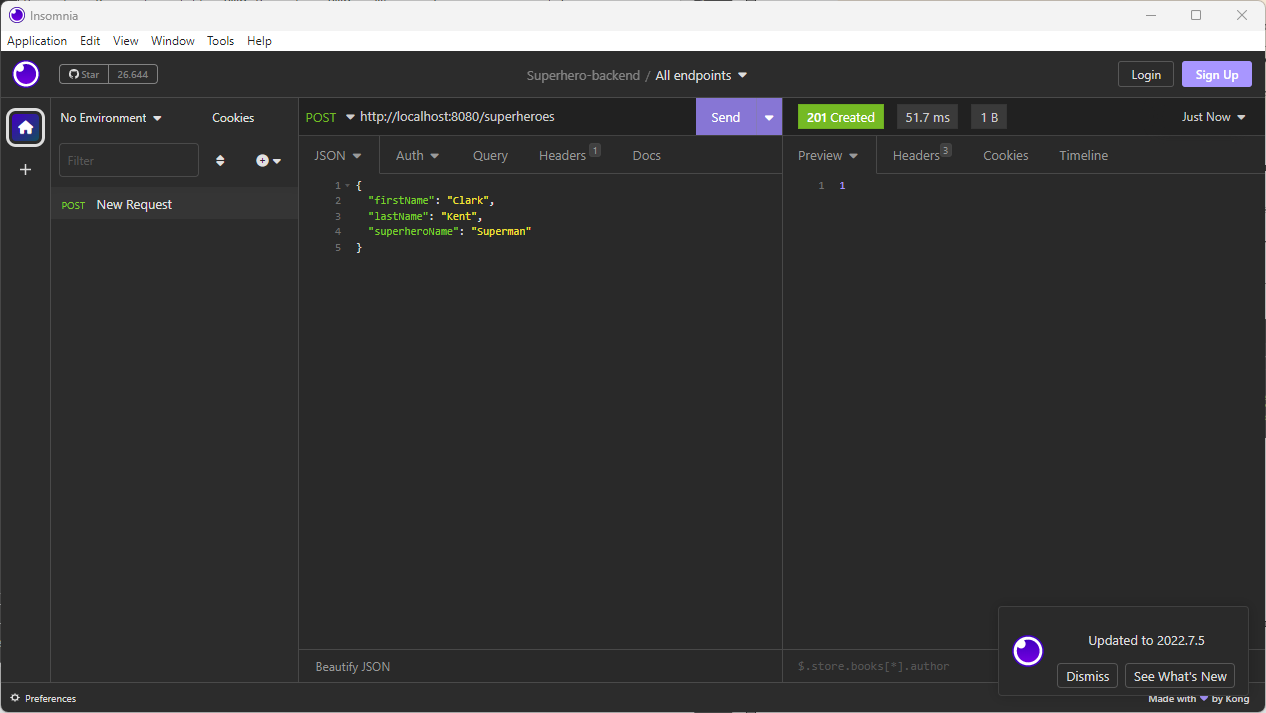
\includegraphics[width=\textwidth]{./images/chapter2/post-request-insomnia.png} 

Look at the method createSuperhero in the class below. The datatype of the parameter is SuperheroRequest and is annotated with @RequestBody.  Therefore the body of the HTTP request in JSON-format is mapped to an object of the class (when the fields correspond). 

The RestController uses the implementation of SuperheroService to map this SuperheroRequest to a Superhero-entity. Finally, the SuperheroRepository is responsible for saving the Superhero-entity in the database. 


\begin{lstlisting}[frame=single]
package be.pxl.superhero.api;

import be.pxl.superhero.service.SuperheroService;
import org.springframework.http.HttpStatus;
import org.springframework.http.ResponseEntity;
import org.springframework.web.bind.annotation.DeleteMapping;
import org.springframework.web.bind.annotation.GetMapping;
import org.springframework.web.bind.annotation.PathVariable;
import org.springframework.web.bind.annotation.PostMapping;
import org.springframework.web.bind.annotation.PutMapping;
import org.springframework.web.bind.annotation.RequestBody;
import org.springframework.web.bind.annotation.RequestMapping;
import org.springframework.web.bind.annotation.RestController;

import java.util.List;

@RestController
@RequestMapping("/superheroes")
public class SuperheroController {

	private final SuperheroService superheroService;

	public SuperheroController(SuperheroService superheroService) {
		this.superheroService = superheroService;
	}

	@GetMapping
	public List<SuperheroDTO> getSuperheroes() {
		return superheroService.findAllSuperheroes();
	}

	@GetMapping("/{superheroId}")
	public SuperheroDTO getSuperheroById(@PathVariable Long superheroId) {
		return superheroService.findSuperheroById(superheroId);
	}
	
	@PostMapping
	public ResponseEntity<Long> createSuperhero(@RequestBody SuperheroRequest superheroRequest) {
		return new ResponseEntity<>(superheroService.createSuperhero(superheroRequest), HttpStatus.CREATED);
	}
	
	@PutMapping("/{superheroId}")
	public SuperheroDTO updateSuperhero(@PathVariable Long superheroId, @RequestBody SuperheroRequest superheroRequest) {
		return superheroService.updateSuperhero(superheroId, superheroRequest);
	}
	
	@DeleteMapping("/{superheroId}")
	public ResponseEntity<Void> deleteSuperhero(@PathVariable Long superheroId) {
		boolean deleted = superheroService.deleteSuperhero(superheroId);
		return deleted? new ResponseEntity<>(HttpStatus.OK) : new ResponseEntity<>(HttpStatus.BAD_REQUEST);
	}
}
\end{lstlisting}

\begin{oefening}
Add @RestController SuperheroController to your Spring Boot application.  Restart the project and create a new superhero with insomnia or postman.  Next you call the REST endpoint to retrieve all superheroes or retrieve the superhero by id. 

Here is the json-format to create a superhero:
\begin{lstlisting}
{
	"firstName": "Clark",
	"lastName": "Kent",
	"superheroName": "Superman"
}
\end{lstlisting}
\end{oefening}

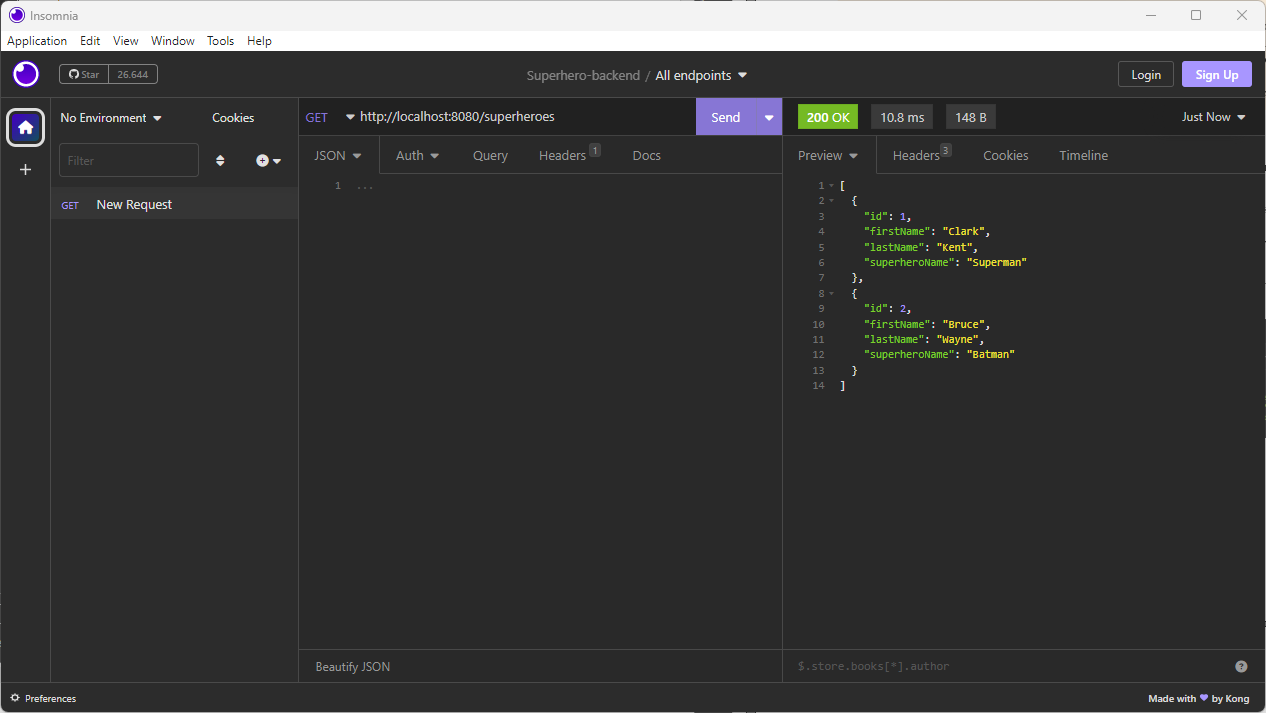
\includegraphics[width=\textwidth]{./images/chapter2/get-request-insomnia.png}

\section{URL context path}

When you want to add a prefix e.g. /api to all the URLs provided by the application, you can add the following key-value-pair in the file application.properties:

\begin{lstlisting}[frame=single]
server.servlet.context-path=/api
\end{lstlisting}


\begin{oefening}
Change the context-path of your Spring Boot application. The prefix /api should be used for the application.  Restart the application and test the endpoints.
\end{oefening}

\section{Resource not found}

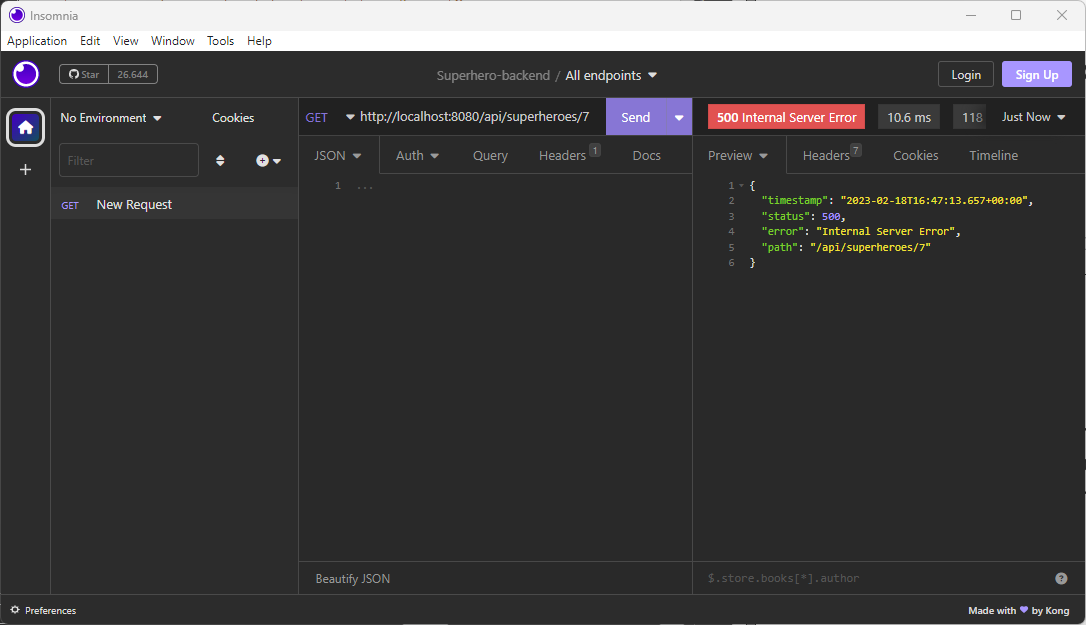
\includegraphics[width=\textwidth]{./images/chapter2/not_found_1.png}

\begin{lstlisting}
package be.pxl.superhero.exception;

import org.springframework.http.HttpStatus;
import org.springframework.web.bind.annotation.ResponseStatus;

@ResponseStatus(HttpStatus.NOT_FOUND)
public class ResourceNotFoundException extends RuntimeException {
    public ResourceNotFoundException(String resource, String field, String value) {
        super("Not found: " + resource + " with " + field + "=" + value);
    }

    public ResourceNotFoundException(String resource, String field, long value) {
        this(resource, field, Long.toString(value));
    }
}
\end{lstlisting}

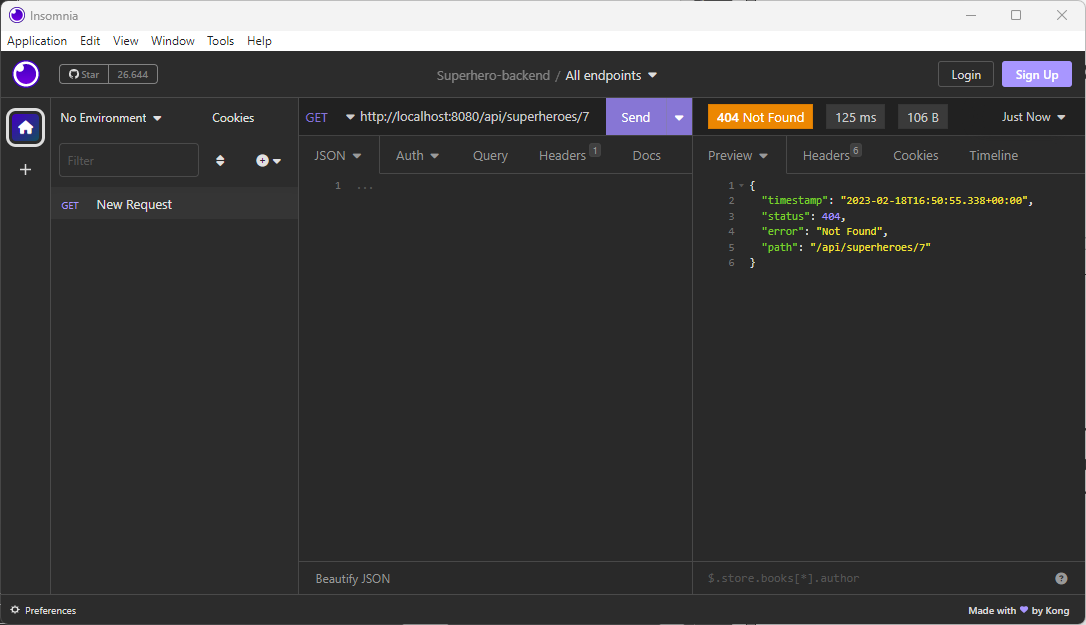
\includegraphics[width=\textwidth]{./images/chapter2/not_found_2.png}

\section{API documentation}

Documentation about your Superhero REST API can be made available with the third-party library. You must add following dependencies to the file pom.xml.

\begin{lstlisting}[language=xml]
<dependency>
	<groupId>org.springdoc</groupId>
	<artifactId>springdoc-openapi-starter-webmvc-ui</artifactId>
	<version>2.0.0</version>
</dependency>
<dependency>
	<groupId>org.springframework.boot</groupId>
	<artifactId>spring-boot-starter-validation</artifactId>
</dependency>
\end{lstlisting}

This documentation in xml-format that can be found by the URL \url{http://localhost:8080/api/v3/api-docs} is not user-friendly.  However, if you open the URL \url{http://localhost:8080/api/swagger-ui.html} in you browser, you can see a user-friendly swagger page where you can even test your API.


\begin{tcolorbox}[colback=blue!5!white,colframe=blue!75!black,title=H2 database]
Our H2 in-memory database disappears when you close the application and all data is lost.
You can use files to permanently save the data.  If you want to inspect the data of your in-memory database, you can add the following property to the file application.properties (located in the resources folder)
\begin{lstlisting}[frame=single]
spring.h2.console.enabled=true
\end{lstlisting}
When you start the Spring Boot application, you are given a unique identifier for your database.  
\begin{lstlisting}[frame=single]
H2 console available at '/h2-console'. Database available at 'jdbc:h2:mem:f5f92e54-3aff-4986-9d00-a0028b0eb6ed'
\end{lstlisting}
When you open the URL \url{http://localhost:8080/api/h2-console} in a browser and fill in the unique id and the username ``sa'' (the password field is left blank),  you are given access to the tables and data of your database. 

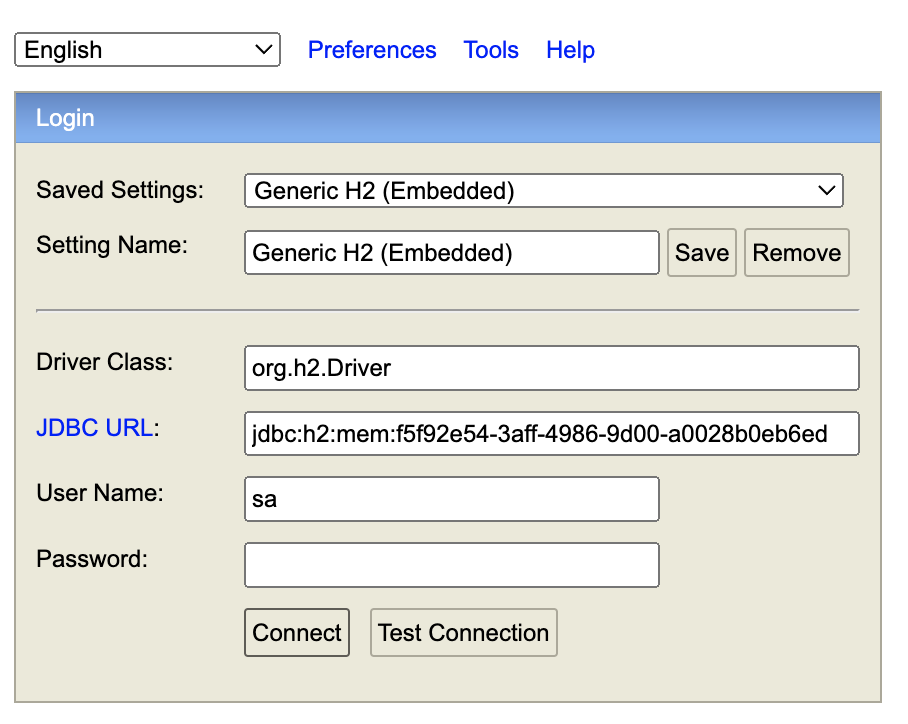
\includegraphics[width=\textwidth]{./images/chapter2/h2-database.png} 

More information about the H2 database is available at \url{https://www.baeldung.com/spring-boot-h2-database}.
\end{tcolorbox}

\section{Frontend}

A frontend for the superhero application written in Angular can be found at github.  (Credits to: \url{https://github.com/shoul10}).


 \fcolorbox{black}[HTML]{ADD8E6}{\parbox{\textwidth}{%
\noindent \textbf{Source code}\\
The frontend code is available at: \url{https://github.com/custersnele/superhero-frontend.git}
}}

Our backend should support CORS to make the API available for the angular frontend.  Cross-origin resource sharing (CORS) is a W3C specification used by most browsers.  

Add the following configuration to your project to support CORS.

\begin{lstlisting}[frame=single]
package be.pxl.superhero.config;

import org.springframework.context.annotation.Configuration;
import org.springframework.web.servlet.config.annotation.CorsRegistry;
import org.springframework.web.servlet.config.annotation.WebMvcConfigurer;

@Configuration
public class WebMvcConfig implements WebMvcConfigurer {
    private static final long MAX_AGE_SECS = 3600;

    @Override
    public void addCorsMappings(CorsRegistry registry) {
        registry.addMapping("/**")
                .allowedOrigins("*")
                .allowedMethods("HEAD", "OPTIONS", "GET", "POST", "PUT", "PATCH", "DELETE")
                .maxAge(MAX_AGE_SECS);        
    }
}
\end{lstlisting}

\begin{oefening}
Add CORS support to your project. The class WebMvcConfig will be located in the package  \textit{be.pxl.superhero.config}.  Restart the Spring Boot application.
Download the frontend code from github and open it in a  development environment (e.g.  WebStorm).  Start the frontend application (ng serve) and create, update and delete your superheroes.
\end{oefening}

\section{Records}

The Java record class type makes DTOs even more easy. It allows us to reduce boilerplate code. 

For example, this record class:

\begin{lstlisting}
package be.pxl.superherobackend.api;

public record SuperheroDTO (Long id, String firstName, String lastName, String superheroName) {
}
\end{lstlisting} 

is equal to this traditional Java class:

\begin{lstlisting}
package be.pxl.superherobackend.api;

public class SuperheroDTO {
    private final Long id;
    private final String firstName;
    private final String lastName;
    private final String superheroName;

    public SuperheroDTOFull(Long id, String firstName, String lastName, String superheroName) {
        this.id = id;
        this.firstName = firstName;
        this.lastName = lastName;
        this.superheroName = superheroName;
    }

    public Long getId() {
        return id;
    }

    public String getFirstName() {
        return firstName;
    }

    public String getLastName() {
        return lastName;
    }

    public String getSuperheroName() {
        return superheroName;
    }

    @Override
    public boolean equals(Object o) {
        if (this == o) return true;
        if (o == null || getClass() != o.getClass()) return false;

        SuperheroDTO that = (SuperheroDTO) o;

        if (id != null ? !id.equals(that.id) : that.id != null) return false;
        if (firstName != null ? !firstName.equals(that.firstName) : that.firstName != null) return false;
        if (lastName != null ? !lastName.equals(that.lastName) : that.lastName != null) return false;
        return superheroName != null ? superheroName.equals(that.superheroName) : that.superheroName == null;
    }

    @Override
    public int hashCode() {
        int result = id != null ? id.hashCode() : 0;
        result = 31 * result + (firstName != null ? firstName.hashCode() : 0);
        result = 31 * result + (lastName != null ? lastName.hashCode() : 0);
        result = 31 * result + (superheroName != null ? superheroName.hashCode() : 0);
        return result;
    }

    @Override
    public String toString() {
        return "SuperheroDTO{" +
                "id=" + id +
                ", firstName='" + firstName + '\'' +
                ", lastName='" + lastName + '\'' +
                ", superheroName='" + superheroName + '\'' +
                '}';
    }
}

\end{lstlisting}

A record class is a concise way to define an object that is shallowly immutable. The values inside a record are called record components. These are declared in the header of the record. Shallowly immutable means that the references that the immutable instance hold cannot change, but the values inside the referred instance can change.

It is possible to override the constructor in a record class.

\begin{oefening}
Replace SuperheroDTO and SuperheroRequest with record classes.  Fix the code and test your application.
\end{oefening}
  


\printbibliography



\end{document}
